
\section{Introduction}

Multi-Component and Multi-Layer Neural Networks (MMNNs), also known as Random Feature and Low-Rank  models (RF-LR), represent a promising
 architecture in scientific machine learning that combines the expressive power of deep networks, capability of fitting high-frequency functions without
 a-priori, and having linear-in-width computational efficiency~\cite{zhang2025structuredbalancedmulticomponentmultilayer}. 
 These architectures introduce low-rank bottlenecks
  at each layer, alternating between wide hidden layers of width \( N \) and narrow bottleneck layers of rank \( r \ll N \), 
  where only the right part of the weights matrices low-rank factorization are trained 
while the right part remain frozen as random ReLU + linear features and RKHS. Hence, we keep the low-rank structural advantage \cite{kamalakara2022exploringlowranktraining} without requiring Riemannian gradient descent.
Recent empirical work by 
 \textit{Zhang et al.}~\cite{zhang2025structuredbalancedmulticomponentmultilayer} has demonstrated that 
 RF-LRs achieve global strong-convergence across a wide range of tasks, including neural-network based PDE solving with and without Physics-Informed losses~\cite{raissi2017physicsinformeddeeplearning}. 
 Training exhibits super convergence with 1st order optimization and a distinctive stepwise loss dynamics, where long plateaus are punctuated by sharp drops.
Despite these empirical successes, a fundamental theoretical understanding of how the loss landscape behaves in RF-LR remains incomplete. The remarkable convergence properties observed in practice—where training displays emergent staircase-like behavior and achieves global minima even when standard neural network training would fail—suggest that the landscape structure of RF-LR differs fundamentally from that of fully-trainable networks. Understanding these landscape properties requires developing a theoretical framework that can explain why RF-LR exhibit such favorable optimization behavior, what drives the stepwise dynamics, and how the low-rank structure shapes the loss surface geometry.

The Neural Tangent Kernel (NTK) framework~\cite{jacot2018neural} provides the natural lens 
for analyzing the early training stage. This perspective has been extended to finite width \cite{huang2019dynamicsdeepneuralnetworks,dyer2019asymptoticswidenetworksfeynman} and large-depth \cite{guillen2025finitewidthneuraltangentkernels,yang2023tensorprogramsvifeature,terjek2022depth}, 
revealing how the Laplacian kernel structure governs the gradient descent (GD) training dynamics and generalization. 
However, applying NTK theory to RF-LR raises new challenges: the low-rank parameterization creates a fundamentally different correlation structure with the same feature map.

We prove that the feature map and RKHS remains the same as in the classical NTK, and hence NTK regimes certifying global convergence can be attained with linear-in-width parameter budget instead of quadratic $O(N^2)$.

By voluntarily putting ourselves in simplifying assumptions (homogeneous activation, isotropic random features, etc.), we are able to derive tractable results on spectrum convergence.
Besides facilitating training, random features assumption keep the kernel structure consistent (Laplacian RKHS from relu feature map) by keeping proofs 
simpler without having to handle more complex correlation structures to bound in the weights. NTK weights do not move during training \cite{jacot2018neural}, so
we fix them and go further.


\subsection*{Low rank architecture }
The considered architecture is a stacking of high then low width layers:
\begin{figure}[htbp]
    \centering
    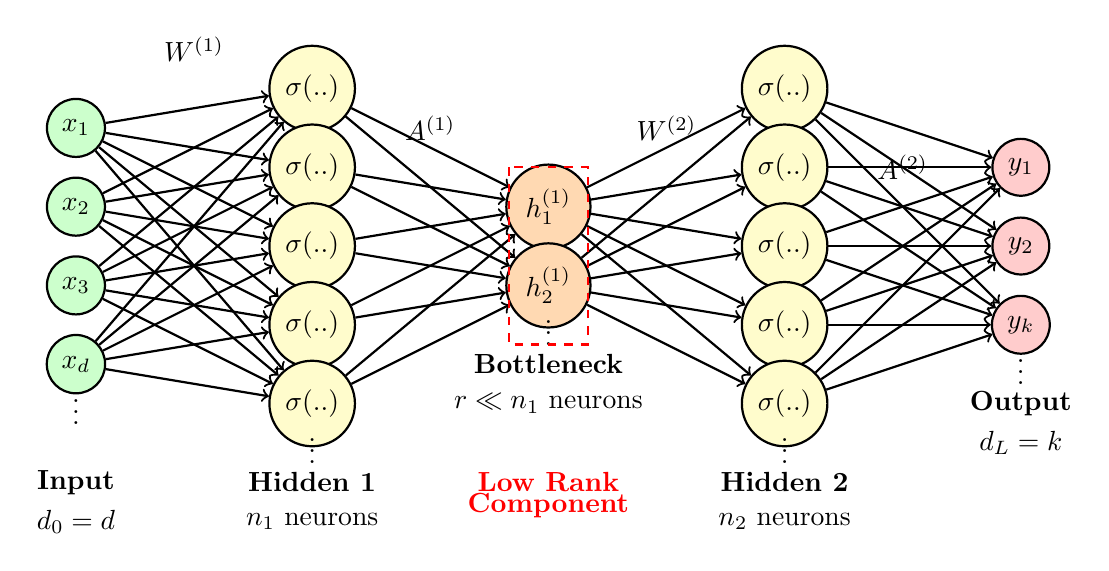
\begin{tikzpicture}[
        node distance=2cm and 3cm,
        neuron/.style={circle, draw, fill=blue!20, minimum size=15pt},
        input/.style={circle, draw, fill=green!20, minimum size=15pt},
        output/.style={circle, draw, fill=red!20, minimum size=15pt},
        hidden/.style={circle, draw, fill=yellow!20, minimum size=15pt},
        bottleneck/.style={circle, draw, fill=orange!30, minimum size=15pt},
        thick
    ]
    % Input layer
    \node[input] (x1) at (0,2) {$x_1$};
    \node[input] (x2) at (0,1) {$x_2$};
    \node[input] (x3) at (0,0) {$x_3$};
    \node[input] (xd) at (0,-1) {$x_d$};
    \node at (0,-1.5) {$\vdots$};
    % First hidden layer
    \node[hidden] (h11) at (3,2.5) {$\sigma(..)$};
    \node[hidden] (h12) at (3,1.5) {$\sigma(..)$};
    \node[hidden] (h13) at (3,0.5) {$\sigma(..)$};
    \node[hidden] (h14) at (3,-0.5) {$\sigma(..)$};
    \node[hidden] (h15) at (3,-1.5) {$\sigma(..)$};
    \node at (3,-2) {$\vdots$};
    % Bottleneck layer (low rank)
    \node[bottleneck] (b1) at (6,1) {$h_1^{(1)}$};
    \node[bottleneck] (b2) at (6,0) {$h_2^{(1)}$};
    \node at (6,-0.5) {$\vdots$};
    % Second hidden layer
    \node[hidden] (h21) at (9,2.5) {$\sigma(..)$};
    \node[hidden] (h22) at (9,1.5) {$\sigma(..)$};
    \node[hidden] (h23) at (9,0.5) {$\sigma(..)$};
    \node[hidden] (h24) at (9,-0.5) {$\sigma(..)$};
    \node[hidden] (h25) at (9,-1.5) {$\sigma(..)$};
    \node at (9,-2) {$\vdots$};
    % Output layer
    \node[output] (y1) at (12,1.5) {$y_1$};
    \node[output] (y2) at (12,0.5) {$y_2$};
    \node[output] (yk) at (12,-0.5) {$y_k$};
    \node at (12,-1) {$\vdots$};
    % Connections input to first hidden
    \foreach \i in {1,2,3,d} {
        \foreach \j in {11,12,13,14,15} {
            \draw[->] (x\i) -- (h\j);
        }
    }
    % Connections first hidden to bottleneck
    \foreach \i in {11,12,13,14,15} {
        \foreach \j in {1,2} {
            \draw[->] (h\i) -- (b\j);
        }
    }
    % Connections bottleneck to second hidden
    \foreach \i in {1,2} {
        \foreach \j in {21,22,23,24,25} {
            \draw[->] (b\i) -- (h\j);
        }
    }
    % Connections second hidden to output
    \foreach \i in {21,22,23,24,25} {
        \foreach \j in {1,2,k} {
            \draw[->] (h\i) -- (y\j);
        }
    }
    % Layer labels
    \node at (0,-2.5) {\textbf{Input}};
    \node at (0,-3) {$d_0 = d$};
    \node at (3,-2.5) {\textbf{Hidden 1}};
    \node at (3,-3) {$n_1$ neurons};
    \node at (6,-1) {\textbf{Bottleneck}};
    \node at (6,-1.5) {$r \ll n_1$ neurons};
    \node at (9,-2.5) {\textbf{Hidden 2}};
    \node at (9,-3) {$n_2$ neurons};
    \node at (12,-1.5) {\textbf{Output}};
    \node at (12,-2) {$d_L = k$};
    % Mathematical notation
    \node at (1.5,3) {$\bm{W}^{(1)}$};
    \node at (4.5,2) {$\bm{A}^{(1)}$};
    \node at (7.5,2) {$\bm{W}^{(2)}$};
    \node at (10.5,1.5) {$\bm{A}^{(2)}$};
    % Highlight low rank structure
    \draw[red, thick, dashed] (5.5,1.5) rectangle (6.5,-0.75);
    \node[red] at (6,-2.5) {\textbf{Low Rank}};
    \node[red] at (6,-2.8) {\textbf{Component}};
    \end{tikzpicture}
    \caption{Architecture of a Multi-component Multi-layer Neural Network (RF-LR). The red dashed connections indicate the low-rank component that reduces dimensionality from $n_1$ to $r \ll n_1$ neurons.
    We \textbf{only train the output weights} $\bm{A}^{(1)}$ and $\bm{A}^{(2)}$.}
    \label{fig:RF-LR_architecture}
\end{figure}




The loss landscape of neural networks plays a crucial role in determining trainability and can assess generalization properties through flatness \cite{li2025seekingconsistentflatminima}. 
Without RKHS advantage, the Laplace kernel's quick spectral decay prevents high-frequency 
learning~\cite{jacot2018neural,cao2020understandingspectralbiasdeep}, while sharp minima can lead to poor
 generalization~\cite{li2018visualizing,fort2019large}. The stepwise loss behavior observed in
  RF-LR~\cite{zhang2025structuredbalancedmulticomponentmultilayer}—where training exhibits long plateaus followed by 
  sharp drops—suggests that the landscape undergoes significant transitions during optimization. By characterizing the NTK 
  spectrum and its evolution, we provide a simpler framework to apply finite-width corrections for understanding these landscape 
  transitions and explaining how the low-rank structure enables the global convergence observed empirically.



  Our approach develops an NTK theory specialized to intra-layers random variables output arising after large-layer acting as gaussian processes, 



\vspace{1em}

\noindent
\textbf{This work addresses the following fundamental questions :}

\vspace{0.3em}

\noindent
\begin{itemize}
\item \emph{How Low-Rank preserves MLPs expressivity and how random features simplify NTK analysis ?}
\end{itemize}
\vspace{0.5em}

This question is closely related to the open question of the curse of dimensionality in deep learning optimization \cite{na2025cursedimensionalityneuralnetwork}.
In particular we show that the curse of dimensionality occuring in the NTK exponential-in-dim spectral decay is not mitigated by low-rank structure.

By exploiting particularities from Fisher and Kibble distributions~\cite{fisher1915probable,hotelling1953new} and manipulation
of non-integer Puiseux polynomials series of correlation-kernels inside expectations, we are able to derive 
the RKHS structure inherent in frozen weights using a characterization from \cite{bietti2021deepequalsshallowrelu}. We focus specifically on the NTK regime where analytical tractability is greatest and the advantages of the 
low-rank random feature structure are most clearly visible.


This work is seminal in further applying Feynman diagrams type computations to finite-width  NTK in the Neural Tangent Hierarchy \cite{dyer2019asymptoticswidenetworksfeynman}, 
because random features allows to remove part of correlations tensors arising in full-rank MLPs 
 , characterize the spectral structure of the kernel matrix, and establish concentration 
 bounds—all while providing insights into how the landscape geometry shapes optimization dynamics.
 Finite-width corrections principal bottleneck arising
 in computating 4-th order neurons correlations in tensors for same layers \cite{guillen2025finitewidthneuraltangentkernels} are simplified
  by non-interacting weights separated by random features.

 
By characterizing the NTK structure, spectral properties for gram matrices coming from datasets, 
and RKHS geometry, we provide the first step towards a theoretical foundation for understanding the favorable optimization dynamics observed empirically. 
Other steps include in future work the mean-field convergence analysis following foundations from \cite{nguyen2023rigorousframeworkmeanfield} and loss-landscape analysis
 with Central Flows \cite{cohen2025understandingoptimizationdeeplearning}. 

 

\vspace{1em}
\subsection{Related work}


The Neural Tangent Kernel (NTK) framework~\cite{jacot2018neural} characterizes infinitely wide neural networks trained by gradient descent as kernel methods 
with a fixed kernel. This framework has been extended to finite width~\cite{arora2019exact}, convolutional architectures~\cite{arora2019harnessing}, and
 depth~\cite{yang2019scaling,terjek2022depth}, establishing a comprehensive theoretical foundation for understanding wide network training. Recent work
  by~\cite{benigni2025eigenvaluedistributionneuraltangent} characterizes the eigenvalue distribution of the NTK in the quadratic scaling regime (width \( N \sim d^2 \)) 
  for single-layer networks, establishing deformed Marchenko–Pastur laws with spike-bulk structure. Their analysis requires careful tracking of correlation diagrams and
   moment calculations. We extend this spectral analysis to the three-layer case with random features, where the rank-\( r \) bottleneck and frozen feature weights 
   fundamentally alter the kernel's spectral properties. A key technical advantage of our approach is that we \textbf{avoid computing correlation diagrams} by
    leveraging the decoupling properties of Fisher–Kibble distributions and the independence structure inherent in frozen random features, which simplifies the 
    analysis while maintaining rigor. Parallel to this, random feature approximations~\cite{rahimi2007random,rahimi2008weighted} provide a practical route to kernel
     approximation by sampling features from suitable distributions, with rigorous guarantees for generalization~\cite{bach2017breaking,rudi2017generalization} and
      approximation~\cite{sriperumbudur2015optimal}. Notably, freezing random features ensures full support for the Barron-space limit in the mean-field regime throughout training, so universal approximation persists 
      at all finite times—a property stronger than classical kernel ridge assumptions. NTK spectrum dependence in depth has been derived in \ work on MLPs at the EOC \cite{terjék2025mlpseocspectrumntk}
      where a linear-in-depth scaling law traduces enhanced training capabilities by stacking layers.

Low-rank and factorized architectures~\cite{sainath2013low,novikov2015tensorizing,arora2018optimization} substantially reduce parameter counts in neural networks. 
However, the training dynamics of factorized weights can differ from unfactorized gradient descent due to implicit regularization effects. When only output weights 
are trained while feature weights remain frozen, the architecture avoids Riemannian geometry complications while achieving linear parameter scaling \( O(rN) \),
 representing an extreme case of factorization that enables clean theoretical analysis.

Neural networks exhibit a well-documented spectral bias toward low frequencies~\cite{rahaman2019spectral,xu2019training}, where low-frequency components are learned
 before high-frequency ones. This bias has been quantified via NTK analysis~\cite{basri2020frequency} and Fourier methods~\cite{tancik2020fourier}, revealing how kernel 
 structure shapes learning dynamics. The "deep equals shallow" result for ReLU kernels in the NTK regime~\cite{bietti2021deepequalsshallowrelu} establishes that the RKHS
  induced by deep networks coincides with that of a shallow ReLU kernel, providing formal NTK spectrum decay rates. The same work characterizes the eigenvalue decay of 
  rotation-invariant kernels on the sphere via endpoint expansions of the kernel \( \kappa(\rho) \) near \( \rho=\pm 1 \), relating the smoothness properties of the kernel at the endpoints to the decay rate of spherical-harmonic eigenvalues. This connection between kernel smoothness and spectral decay provides a principled framework for understanding how RKHS structure, kernel spectra, and training behavior interact.

Multi-index approaches~\cite{benarous2021online,damian2022neural,abbe2023sgd} learn functions of the form \( f(x)=\sum_{j=1}^r g_j(\langle v_j,x\rangle) \) by 
discovering latent directions sequentially, with training displaying staircase dynamics featuring plateaus for inactive directions. In extensive-rank regimes 
\( r\asymp d^\beta \), these works derive scaling laws~\cite{damian2022neural} that connect rank, dimension, and sample complexity. three-layer RF-LR sees their mid layer
acting as having \(r\) independent functions (approximated by the random features basis) forming a multi-index model in function space. Those functions only 
interact through reconstructing output functions in next layers. This point of view is a novel way to understand low rank weight matrices provided
that you do not train the random features to ensure approximation of dictionary - reconstruction - approxim .. etc ..

From a data-dependent scaling perspective, achieving and maintaining NTK behavior in fully-trainable deep networks can impose stringent width–data 
requirements, often quoted in the literature as polynomial \( O(N^p) \) in the width \( N \), with worst-case exponents \( p = 4\), and best-case exponents \( p = 1\) \cite{nguyen2022tightboundssmallesteigenvalue}
for quadratic scaling. To ensure the NTK has a positive smallest eigenvalue—crucial for optimization 
 convergence—at least one layer must scale with the number of data samples \( n \), while other layers can scale arbitrarily up to logarithmic
 factors for deep networks, motivating architectures that achieve NTK regime behavior with tractable computational requirements for large scale applications.


\subsection*{Our Contributions}
Our contributions are: (i) an NTK recursion specialized to RF-LR together with finite-width corrections and concentration rates, (ii) a three-layer spectral theory yielding a signal–noise decomposition of the empirical kernel and a deformed MP law with a spike for the kernel matrix spectrum, and (iii) a principled argument—grounded in~\cite{bietti2021deepequalsshallowrelu}—that RF-LR suffers no RKHS disadvantage relative to deep fully-trainable networks. These theoretical results are complemented by numerical experiments (omitted here) that verify NTK spectral concentration, staircase loss dynamics, and the scaling benefits of RF-LR at moderate widths.

More specifically:
\begin{itemize}
    \item \textbf{NTK recursion} We derive the new NTK recursion expansion for RF-LR (\( \sigma_A, \sigma_c, \beta = 1 \)), yielding clean expressions for three-layer and general \( L \)-layer networks.
    \item \textbf{RKHS Preserved} In the NTK regime \( f_t(x)\!\approx\! f_0(x)+\langle\nabla_\theta f_0(x),\,\theta_t-\theta_0\rangle \) and \( f_t\in\mathcal{H}_\Theta \) with \( \|f\|_{\mathcal{H}_\Theta}^2=\langle f,\Theta^{-1}f\rangle_{L^2} \). RF‑LR preserves universal approximation (frozen Gaussian \( w^{(\ell)} \)), the rank‑\(r\) bottleneck acts as a spectral filter, and its NTK‑RKHS has the same decay rate as an MLP's while using \(O(rN)\) rather than \(O(N^2)\) parameters.
    \item \textbf{Marcheko-Pastur like Gram spectrum (three-layer case).} We state and analyze Fisher–Kibble decoupling~\cite{fisher1915probable,hotelling1953new}, a signal–noise decomposition of the empirical NTK, and a deformed Marchenko–Pastur law (with spike) for the kernel matrix spectrum under standard random matrix scaling.
\end{itemize}
